%% RAVA -- revised manuscript (IEEEtran journal)
\documentclass[journal]{IEEEtran}
\usepackage{cite}
\usepackage{amsmath,amssymb,amsfonts}
\usepackage{amsthm}
\usepackage{algorithm}
\usepackage[noend]{algpseudocode}
\usepackage{graphicx}
\usepackage{booktabs}
\usepackage{multirow}
\usepackage{array}
\usepackage{xcolor}
\usepackage{pifont}
\usepackage[most]{tcolorbox}
\usepackage{tikz}
\usetikzlibrary{arrows.meta,positioning,fit,calc,backgrounds,shapes.misc}
\usepackage[hidelinks]{hyperref}
\usepackage[capitalise,nameinlink]{cleveref}

\definecolor{ravablue}{HTML}{1F5FBF}
\definecolor{ravagrey}{HTML}{555555}
\definecolor{ravalight}{HTML}{E8EEF8}
\newcommand{\cmark}{\ding{51}}
\newcommand{\xmark}{\ding{55}}
\newtcolorbox{keybox}[1]{enhanced, colback=ravalight, colframe=ravablue, boxrule=0.6pt, arc=2pt,
  left=4pt, right=4pt, top=3pt, bottom=3pt, fonttitle=\bfseries\small, title=#1, fontupper=\small}

\newtheorem{lemma}{Lemma}
\newtheorem{theorem}{Theorem}
\newtheorem{proposition}{Proposition}
\newtheorem{corollary}{Corollary}
\newtheorem{assumption}{Assumption}
\newtheorem{definition}{Definition}
\theoremstyle{remark}
\newtheorem{remark}{Remark}
\algrenewcommand\algorithmicrequire{\textbf{Input:}}
\algrenewcommand\algorithmicensure{\textbf{Output:}}
\crefname{algorithm}{Algorithm}{Algorithms}
\crefname{assumption}{Assumption}{Assumptions}
\crefname{definition}{Definition}{Definitions}

\newcommand{\E}{\mathbb{E}}
\newcommand{\R}{\mathbb{R}}
\newcommand{\gk}{g_\kappa}

\begin{document}
\title{RAVA: A Reciprocal Adaptive Value and Resource Allocation Auction for Reliability-Aware GPU and Cloud Clusters}
\author{Firstname~Lastname,~\IEEEmembership{Member,~IEEE},
        and~Firstname~Lastname%
\thanks{Manuscript received November 19, 2026. (Corresponding author: Firstname Lastname.)}%
\thanks{The authors are with the Department of Computer Science and Engineering, University Name, City, Country (e-mail: author@university.edu).}%
\thanks{Source code, traces-processing scripts, raw results and the Slurm broker are provided in the accompanying artifact.}}
\markboth{IEEE Transactions on Parallel and Distributed Systems,~Vol.~XX, No.~X, Month~2026}%
{Lastname \MakeLowercase{\textit{et al.}}: RAVA: Reciprocal Adaptive Value and Resource Allocation Auction}
\maketitle

\begin{abstract}
Most auctions for shared clusters give resources to the highest bidder. But a winner may never use what it wins, and then GPUs sit idle. We propose RAVA, the Reciprocal Adaptive Value and Resource Allocation Auction. RAVA scores each bid by the user's measured reliability, job size, past efficiency and timing flexibility. It packs jobs onto servers in score order and charges each winner the lowest bid that would still have won. Winners pay only if their job runs; no-shows forfeit a deposit. We show that this settlement rule implies one correct reliability factor, $g_\kappa(\rho)=\rho+(1-\rho)\kappa$, and that the naive factor $\rho$ double-counts risk. We prove that honest bidding is dominant in each round and nearly dominant over many rounds, with a gap that shrinks as reputation history grows. We also bound the damage of users who build a reputation and then default. We evaluate RAVA on 59 days of the Microsoft Philly GPU trace, with real job outcomes and gang scheduling on 8-GPU servers, and on 200 synthetic workloads. We compare it with eight mechanisms, including G-VMPAC, online primal-dual pricing and overbooking. On held-out Philly days RAVA beats LOS by 6.4\% (95\% CI 3.4--9.4\%, Holm $p<0.001$) and ties overbooking. Combined with overbooking it reaches 91.1\% of an oracle bound. RAVA runs 10{,}000 jobs in 3.1\,s and runs live on Slurm. Its gain vanishes when few resources are lost to failures.
\end{abstract}

\begin{IEEEkeywords}
Mechanism design, auctions, GPU clusters, cloud computing, reputation, truthfulness, Slurm, resource allocation.
\end{IEEEkeywords}

%=====================================================================
\section{Introduction}
%=====================================================================
\IEEEPARstart{G}{PU} clusters are expensive and shared by many teams. Clouds, universities and AI labs all face one question: who gets which GPUs, and when? Many systems answer with auctions~\cite{buyya2002,luong2017,parsons2011,mahajan2020themis}. Users bid, and the auction picks winners and prices.

Classic auctions give resources to the users who pay most. In a cluster this hides a cost: \emph{a winner may not use what it wins}. Jobs crash, inputs are late, and users cancel. In the Microsoft Philly trace~\cite{jeon2019philly}, 28\% of jobs did not pass. In our evaluation window, those jobs held 57\% of the GPU-hours (\cref{sec:philly}). First-price, second-price and VCG auctions~\cite{vickrey1961,clarke1971,groves1973} treat every winning bid as delivered value. So they can fill a cluster with work that never finishes.

This paper asks: \emph{how should an auction price the risk that a winner will not run, without losing truthfulness or speed?} We answer with \emph{RAVA}.

\begin{keybox}{RAVA in five lines}
\begin{itemize}\setlength\itemsep{1pt}
\item Score $=$ bid $\times$ \textbf{reliability factor} $\times$ efficiency $\times$ flexibility $/\,$\textbf{size}$^{\alpha}$.
\item Fill servers in score order; each winner pays its \textbf{critical bid}.
\item Pay \textbf{only if the job runs}; a no-show forfeits a deposit $\kappa p$.
\item The reliability factor that matches this rule is $g_\kappa(\rho)=\rho+(1-\rho)\kappa$.
\item Reputation and prices change \textbf{only between rounds}.
\end{itemize}
\end{keybox}

\textbf{Contributions.}
\begin{enumerate}
\item \emph{A consistent utility model.} We define a pay-on-use settlement with deposits. We derive each tenant's effective value and the one reliability factor that ranks jobs by expected value (\cref{lem:eff,prop:rank}). We show that the naive factor $\rho$ double-counts risk, and that $\kappa=0$ is the only deposit rate that ranks exactly under every belief.
\item \emph{Multi-round incentive guarantees.} Reputation links rounds, so a user might overbid today to build reputation. We prove that honest bidding is $\varepsilon$-dominant with explicit $\varepsilon$ (\cref{thm:multi}). With forgetting factor $\zeta<1$, a user who builds a reputation and then defaults can do so only a bounded number of times (\cref{prop:exploit}). We also state when whitewashing pays (\cref{prop:white}).
\item \emph{Real traces and GPU-specific scheduling.} We replay 59 days of the Philly trace with real outcomes, per-user history, measured GPU utilization and gang placement on 2- and 8-GPU servers (\cref{sec:philly}).
\item \emph{Strong baselines and statistics.} We compare against G-VMPAC~\cite{nejad2015}, online primal-dual pricing~\cite{zhang2017ton}, overbooking~\cite{qi2025ohtrust}, DRF~\cite{ghodsi2011}, LOS~\cite{lehmann2002}, VCG, McAfee, first- and second-price auctions. We use paired Wilcoxon tests with Holm correction, bootstrap intervals and effect sizes.
\item \emph{Adversaries and scale.} We test bid and window lies, build-then-exploit, whitewashing, unreliable populations up to 60\%, and markets up to 10{,}000 jobs.
\item \emph{A working Slurm broker.} RAVA runs on a live Slurm cluster and settles payments from Slurm's own job records (\cref{sec:slurm}).
\end{enumerate}

We report results as measured. RAVA does not win everywhere. Exact VCG packs better on small markets, overbooking ties RAVA on Philly, and RAVA's gain disappears when failures waste few resources.

%=====================================================================
\section{Related Work}\label{sec:related}
%=====================================================================
\subsection{Truthful Auctions}
Vickrey showed that a second-price auction makes honest bidding dominant~\cite{vickrey1961}. VCG extends this to many items~\cite{clarke1971,groves1973}. Myerson showed that a monotone allocation with critical prices is truthful for single-parameter agents~\cite{myerson1981}; RAVA uses this result. Winner determination for bundles is NP-hard~\cite{sandholm2002,cramton2006}, and VCG has known practical problems~\cite{ausubel2006,rothkopf2007}. Algorithmic mechanism design asks for truthful \emph{and} fast mechanisms~\cite{nisan2001,nisan2007agt}. LOS greedy is one~\cite{lehmann2002}; others build on monotone algorithms or LP relaxations~\cite{archer2001,mualem2008,lavi2011}.

\subsection{Cloud and Cluster Auctions}
Nejad, Mashayekhy and Grosu designed truthful greedy mechanisms for VM provisioning with several resource types, ranking users by bid density with relevance factors~\cite{nejad2015}. Zhang \emph{et al.} built online auctions in IaaS clouds from a primal-dual framework, with prices from dual variables~\cite{zhang2017ton}; such exponential pricing follows Buchbinder and Naor~\cite{buchbinder2009}. Other work studies randomized and online VM auctions~\cite{zhang2014,shi2014}, combinatorial double auctions~\cite{samimi2016}, spot prices~\cite{benyehuda2013}, and edge markets~\cite{luong2017,qiu2021}. McAfee's double auction is truthful and budget-balanced but gives up some trades~\cite{mcafee1992,myerson1983}.

\subsection{GPU Cluster Schedulers}
Themis lets ML jobs bid for GPUs in a partial-allocation auction and targets finish-time fairness~\cite{mahajan2020themis}. Shockwave extends market theory to jobs whose needs change during training~\cite{zheng2023shockwave}. DRF shares several resources fairly without prices~\cite{ghodsi2011}. These systems handle placement and fairness well. None prices the risk that a winner will not run. Jeon \emph{et al.} analyzed the Philly trace that we use~\cite{jeon2019philly}.

\subsection{Reliability, Reputation and Overbooking}
Reputation systems estimate who keeps promises~\cite{resnick2000,josang2002}. Xiao \emph{et al.} use bandit-based reputation to pick reliable sellers in vehicular edge networks~\cite{xiao2023mab}. Oh-Trust overbooks an edge server, with a 10\% overbooking rate in its evaluation, and renews contracts using a learned reputation update~\cite{qi2025ohtrust}. Overbooking is the main alternative to RAVA, so we test it as a baseline and in combination. Online mechanism design gives truthfulness when users cannot report earlier arrivals or later deadlines~\cite{hajiaghayi2004,porter2004}. HPC backfilling reuses idle reservations~\cite{lifka1995,mualem2001}.

\begin{table*}[!t]
\caption{Novelty Comparison With Closest Work (\cmark\ addressed, \xmark\ not addressed, --- not applicable or not stated)}\label{tab:novel}
\centering\footnotesize\setlength{\tabcolsep}{3.2pt}
\begin{tabular}{@{}lcccccccc@{}}
\toprule
Work & Truthful & Multi-resource & GPU servers, & Prices risk of & Multi-round & Polynomial & Real & System\\
 & (DSIC) & + time windows & gang jobs & non-use & incentive bound & time & trace & prototype\\
\midrule
VCG~\cite{clarke1971,groves1973} & \cmark & \cmark & --- & \xmark & \xmark & \xmark & --- & ---\\
LOS~\cite{lehmann2002} & \cmark & bundles & \xmark & \xmark & \xmark & \cmark & --- & ---\\
G-VMPAC~\cite{nejad2015} & \cmark & resources & \xmark & \xmark & \xmark & \cmark & --- & ---\\
Online primal-dual~\cite{zhang2017ton} & \cmark & \cmark & \xmark & \xmark & \xmark & \cmark & \cmark & ---\\
Themis~\cite{mahajan2020themis} & \cmark & GPUs & \cmark & \xmark & fairness only & \cmark & \cmark & \cmark\\
Shockwave~\cite{zheng2023shockwave} & \xmark & GPUs & \cmark & \xmark & \xmark & --- & \cmark & \cmark\\
Oh-Trust~\cite{qi2025ohtrust} & --- & --- & \xmark & overbooking & \xmark & --- & \cmark & ---\\
Xiao \emph{et al.}~\cite{xiao2023mab} & --- & \xmark & \xmark & reputation & \xmark & --- & --- & ---\\
\textbf{RAVA (this work)} & \cmark & \cmark & \cmark & \cmark & \cmark & \cmark & \cmark & \cmark\ (Slurm)\\
\bottomrule
\end{tabular}
\end{table*}

\Cref{tab:novel} summarizes the gap. To our knowledge, RAVA is the first mechanism that combines truthful critical prices, multi-resource gang placement, explicit pricing of non-use under a stated settlement rule, and incentive bounds across rounds.

%=====================================================================
\section{System Model}\label{sec:model}
%=====================================================================
\begin{figure*}[!t]
\centering
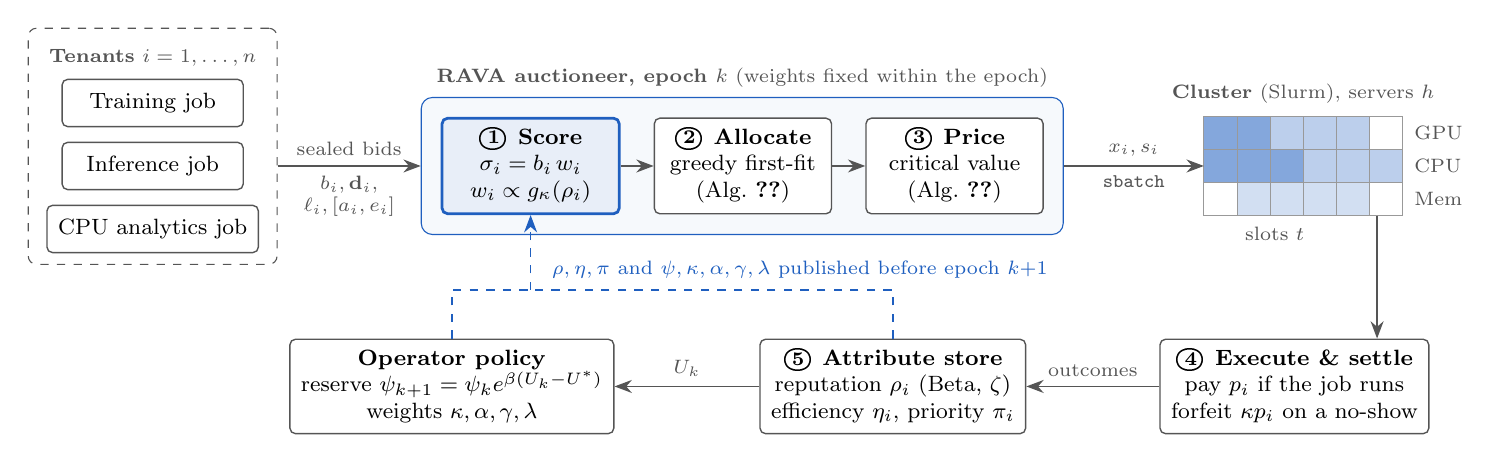
\begin{tikzpicture}[
  font=\footnotesize, >={Stealth[length=2.2mm]},
  box/.style={draw=ravagrey, rounded corners=2pt, align=center, inner sep=4pt, line width=0.5pt},
  stp/.style={box, fill=white, minimum width=2.25cm, minimum height=1.05cm},
  acc/.style={stp, draw=ravablue, line width=1pt, fill=ravalight},
  lab/.style={font=\scriptsize, text=ravagrey, align=center},
  flow/.style={->, line width=0.6pt, draw=ravagrey}]
% tenants
\node[box, minimum width=2.3cm, minimum height=0.6cm] (t1) at (-0.5,1.15) {Training job};
\node[box, minimum width=2.3cm, minimum height=0.6cm] (t2) at (-0.5,0.35) {Inference job};
\node[box, minimum width=2.3cm, minimum height=0.6cm] (t3) at (-0.5,-0.45) {CPU analytics job};
\node[lab, above=1pt of t1] (tl) {\textbf{Tenants} $i=1,\dots,n$};
\node[draw=ravagrey, dashed, rounded corners=3pt, fit=(t1)(t2)(t3)(tl), inner sep=4pt] (T) {};
% auctioneer
\node[acc] (s1) at (4.3,0.35) {\textbf{\textcircled{\scriptsize 1} Score}\\$\sigma_i=b_i\,w_i$\\$w_i\propto g_\kappa(\rho_i)$};
\node[stp, right=0.42cm of s1] (s2) {\textbf{\textcircled{\scriptsize 2} Allocate}\\greedy first-fit\\(Alg.~\ref{alg:alloc})};
\node[stp, right=0.42cm of s2] (s3) {\textbf{\textcircled{\scriptsize 3} Price}\\critical value\\(Alg.~\ref{alg:pay})};
\begin{scope}[on background layer]
\node[draw=ravablue, fill=ravablue!4, rounded corners=4pt, fit=(s1)(s2)(s3), inner sep=7pt, label={[lab, anchor=south]north:\textbf{RAVA auctioneer, epoch $k$} (weights fixed within the epoch)}] (A) {};
\end{scope}
\draw[flow] (T.east |- A.west) -- node[lab, above]{sealed bids} node[lab, below, align=center]{$b_i,\mathbf{d}_i,$\\$\ell_i,[a_i,e_i]$} (A.west);
\draw[flow] (s1) -- (s2); \draw[flow] (s2) -- (s3);
% cluster grid
\begin{scope}[shift={(12.85,-0.28)}]
  \foreach \x in {0,...,5}{\foreach \y in {0,1,2}{\draw[ravagrey!60, line width=0.3pt, fill=white] (\x*0.42,\y*0.42) rectangle ++(0.42,0.42);}}
  \fill[ravablue!55] (0,0.84) rectangle (0.84,1.26); \fill[ravablue!30] (0.84,0.84) rectangle (2.10,1.26);
  \fill[ravablue!55] (0,0.42) rectangle (1.26,0.84); \fill[ravablue!30] (1.26,0.42) rectangle (2.52,0.84);
  \fill[ravablue!20] (0.42,0) rectangle (2.10,0.42);
  \foreach \x in {0,...,5}{\foreach \y in {0,1,2}{\draw[ravagrey!60, line width=0.3pt] (\x*0.42,\y*0.42) rectangle ++(0.42,0.42);}}
  \node[lab, anchor=west] at (2.55,1.05) {GPU}; \node[lab, anchor=west] at (2.55,0.63) {CPU}; \node[lab, anchor=west] at (2.55,0.21) {Mem};
  \node[lab, anchor=north] at (0.9,-0.02) {slots $t$};
  \coordinate (Cw) at (0,0.63);
  \coordinate (Cd) at (2.2,0);
  \node[lab, anchor=south] at (1.26,1.30) {\textbf{Cluster} (Slurm), servers $h$};
\end{scope}
\draw[flow] (A.east) -- node[lab, above]{$x_i,s_i$} node[lab, below]{\texttt{sbatch}} (Cw);
% bottom row
\node[box, minimum width=3.3cm, minimum height=0.95cm] (tel) at (14.0,-2.45) {\textbf{\textcircled{\scriptsize 4} Execute \& settle}\\pay $p_i$ if the job runs\\forfeit $\kappa p_i$ on a no-show};
\node[box, minimum width=3.3cm, minimum height=0.95cm] (rep) at (8.9,-2.45) {\textbf{\textcircled{\scriptsize 5} Attribute store}\\reputation $\rho_i$ (Beta, $\zeta$)\\efficiency $\eta_i$, priority $\pi_i$};
\node[box, minimum width=3.3cm, minimum height=0.95cm] (pol) at (3.3,-2.45) {\textbf{Operator policy}\\reserve $\psi_{k+1}=\psi_k e^{\beta(U_k-U^*)}$\\weights $\kappa,\alpha,\gamma,\lambda$};
\draw[flow] (Cd) -- (Cd |- tel.north);
\draw[flow] (tel.west) -- node[lab, above]{outcomes} (rep.east);
\draw[flow] (rep.west) -- node[lab, above]{$U_k$} (pol.east);
\coordinate (M) at ($(s1.south)+(0,-0.95)$);
\draw[line width=0.6pt, dashed, draw=ravablue] (rep.north) |- (M);
\draw[line width=0.6pt, dashed, draw=ravablue] (pol.north) |- (M);
\draw[flow, dashed, draw=ravablue] (M) -- (s1.south);
\node[lab, text=ravablue, anchor=south west] at ($(M)+(0.15,0.02)$) {$\rho,\eta,\pi$ and $\psi,\kappa,\alpha,\gamma,\lambda$ published before epoch $k{+}1$};
\end{tikzpicture}
\caption{RAVA system. Tenants send sealed bids. RAVA scores, allocates and prices them with weights fixed for the epoch (steps 1--3) and submits winners to Slurm at their slot. After execution it settles on use and updates reputation (steps 4--5); new values are published before the next epoch (dashed).}
\label{fig:arch}
\end{figure*}

\Cref{fig:arch} shows the system and \cref{tab:notation} lists the symbols. One operator runs a cluster of servers $\mathcal{H}$. Tenants bid in rounds, called epochs, indexed by $k$.

\begin{table}[!t]
\caption{Notation}\label{tab:notation}
\centering\footnotesize
\begin{tabular}{@{}ll@{}}
\toprule
Symbol & Meaning\\
\midrule
$\mathcal{H}$, $C_{h,r}$ & servers; capacity of resource $r\in\{1..m\}$ on server $h$\\
$T$, $t$ & slots per epoch; slot index\\
$\mathbf{d}_i, K_i, \ell_i$ & per-server demand, gang size (servers), length\\
$[a_i,e_i]$ & allowed window (earliest start, last slot)\\
$D_i$ & normalized footprint, \eqref{eq:footprint}\\
$v_i$ & value if the job runs (private)\\
$q_i$, $\hat q_i$ & true run probability; tenant's belief\\
$\theta_i$ & effective value, \eqref{eq:theta}; $b_i$ bid\\
$\kappa\in[0,1]$ & deposit rate (forfeited on a no-show)\\
$\rho_i$ & reputation (operator's estimate of $q_i$)\\
$g_\kappa(\rho)$ & reliability factor, $\rho+(1-\rho)\kappa$\\
$\eta_i,\varphi_i,\pi_i$ & efficiency, flexibility, public priority\\
$\alpha,\gamma,\lambda$ & size, efficiency and flexibility weights\\
$w_i$, $\sigma_i$ & weight and score, \eqref{eq:score}\\
$a_0,b_0$; $\zeta$; $\rho_{\min}$ & Beta prior; forgetting factor; reputation floor\\
$\psi$ & reserve price per normalized unit\\
$x_i, s_i, p_i$ & win indicator, start slot, critical price\\
$\delta$ & tenants' discount factor across epochs\\
\bottomrule
\end{tabular}
\end{table}

\subsection{Resources and Jobs}
Server $h$ has capacity $C_{h,r}$ of resource $r$ in each slot $t\in\{1,\dots,T\}$. Job $i$ needs $\mathbf{d}_i\in\R_+^m$ on each of $K_i$ servers, for $\ell_i$ consecutive slots inside $[a_i,e_i]$. A gang job ($K_i>1$) must start on all its servers at once. An allocation gives each winner a start $s_i$ and a server set $H_i$ with $|H_i|=K_i$. No server is over-booked in any slot:
\begin{equation}\label{eq:cap}
\sum_{i:\,h\in H_i,\; s_i\le t<s_i+\ell_i} d_{ir}\le C_{h,r}\qquad\forall h,t,r.
\end{equation}
The footprint of a job is its share of the cluster over time,
\begin{equation}\label{eq:footprint}
D_i=\ell_i K_i\sum_{r=1}^m \frac{d_{ir}}{\sum_{h}C_{h,r}}.
\end{equation}

\subsection{Settlement Rule and Utilities}
A job that wins may still not run. Let $q_i$ be the true chance that it runs, and $\hat q_i$ the tenant's own belief.

\begin{definition}[Pay-on-use with deposit]\label{def:settle}
A winner with price $p_i$ pays $p_i$ if its job runs. If it does not run, the tenant forfeits $\kappa p_i$, where $\kappa\in[0,1]$ is public.
\end{definition}

A tenant gains $v_i$ only if its job runs. Its expected utility from winning at price $p$ is therefore
\begin{equation}\label{eq:util}
u_i(p)=\hat q_i v_i-p\big(\hat q_i+(1-\hat q_i)\kappa\big).
\end{equation}

\begin{lemma}[Effective value]\label{lem:eff}
Under \cref{def:settle}, a tenant wants to win at price $p$ if and only if $p\le\theta_i$, where
\begin{equation}\label{eq:theta}
\theta_i=\frac{\hat q_i v_i}{\hat q_i+(1-\hat q_i)\kappa}.
\end{equation}
\end{lemma}
\begin{proof}
By \eqref{eq:util}, $u_i(p)\ge0$ exactly when $p(\hat q_i+(1-\hat q_i)\kappa)\le\hat q_iv_i$.
\end{proof}
So each tenant is a single-parameter agent with type $\theta_i$. With $\kappa=0$, $\theta_i=v_i$. With $\kappa=1$, $\theta_i=\hat q_iv_i$: the tenant prices its own risk.

\subsection{Operator Information and Goal}
The operator observes each tenant's past outcomes, never its beliefs. It keeps a Beta reputation with forgetting~\cite{josang2002}. After each epoch in which tenant $i$ won, $s_i\gets\zeta s_i+\mathbf{1}[\text{ran}]$ and $f_i\gets\zeta f_i+\mathbf{1}[\text{no-show}]$. Then
\begin{equation}\label{eq:rho}
\rho_i=\max\!\Big(\rho_{\min},\;\frac{a_0+s_i}{a_0+b_0+s_i+f_i}\Big).
\end{equation}
The operator also measures efficiency $\eta_i$ (the share of reserved resources a tenant actually used), and flexibility $\varphi_i=(e_i-a_i+1-\ell_i)/(e_i-a_i+1)$. Its goal is expected value of work that runs:
\begin{equation}\label{eq:obj}
\max_{\mathbf{x},\mathbf{s},H}\;\E[SW]=\sum_i x_i\,q_i\,v_i\quad\text{s.t.~\eqref{eq:cap}}.
\end{equation}

\subsection{Assumptions}
\begin{assumption}\label{as:quasi}
Tenants are single-minded, risk-neutral and quasi-linear.
\end{assumption}
\begin{assumption}\label{as:public}
$\rho_i,\eta_i,\pi_i,\kappa$ and all weights are fixed and published before an epoch opens.
\end{assumption}
\begin{assumption}[Limited misreports~\cite{hajiaghayi2004,porter2004}]\label{as:window}
A job cannot start before its inputs exist. Outputs are released only at the reported deadline. Containers enforce the reported demand.
\end{assumption}
\begin{assumption}\label{as:collusion}
Tenants do not collude, as for LOS and VCG~\cite{lehmann2002,rothkopf2007}.
\end{assumption}
\begin{assumption}[Private outcomes]\label{as:private}
Other tenants' strategies do not depend on tenant $i$'s private outcome history.
\end{assumption}
\begin{assumption}[Bounded values]\label{as:bounded}
Effective values lie in $[0,\bar V]$.
\end{assumption}

%=====================================================================
\section{The RAVA Mechanism}\label{sec:mech}
%=====================================================================
\subsection{Score}
RAVA turns bid $b_i$ into a score $\sigma_i=b_iw_i$ with
\begin{equation}\label{eq:score}
w_i=\frac{\pi_i\,g_\kappa(\rho_i)\,\eta_i^{\gamma}\,(1+\lambda\varphi_i)}{D_i^{\alpha}},\qquad g_\kappa(\rho)=\rho+(1-\rho)\kappa.
\end{equation}
The weight $w_i$ does not depend on $b_i$. The factor $g_\kappa$ is the key change from earlier work: it matches \cref{def:settle} (\cref{prop:rank}). $D_i^{-\alpha}$ scales down large jobs; $\alpha=\tfrac12$ gives the LOS ranking~\cite{lehmann2002}, and $\alpha=1$ ranks by value per unit of capacity, as in G-VMPAC-II~\cite{nejad2015}. $\eta_i^\gamma$ rewards efficient use. $1+\lambda\varphi_i$ rewards disclosed slack. A bid is eligible only if $b_i\ge\psi D_i$.

\subsection{Allocation}
\Cref{alg:alloc} sorts eligible bids by score. Each job takes the earliest start in its window at which $K_i$ servers have room for all $\ell_i$ slots. Among those servers it picks the tightest fit, which limits GPU fragmentation.

\begin{algorithm}[!t]
\caption{RAVA-Allocate}\label{alg:alloc}
\begin{algorithmic}[1]
\Require bids $b_i$; jobs $(\mathbf{d}_i,K_i,\ell_i,a_i,e_i)$; attributes $\rho_i,\eta_i,\pi_i$; capacities $C_{h,r}$; parameters $\kappa,\alpha,\gamma,\lambda,\psi$
\Ensure winners $x_i$, starts $s_i$, server sets $H_i$
\State $\mathcal{E}\gets\{i:b_i\ge\psi D_i\}$; compute $w_i$ by \eqref{eq:score}; $\sigma_i\gets b_iw_i$
\State sort $\mathcal{E}$ by $\sigma_i$, highest first (ties: lower index)
\State $R_{h,t,r}\gets C_{h,r}$ for all $h,t,r$
\ForAll{$i\in\mathcal{E}$ in order}
  \For{$s=a_i$ \textbf{to} $e_i-\ell_i+1$}
    \State $F\gets\{h: R_{h,t}\ge\mathbf{d}_i\ \forall t\in[s,s+\ell_i)\}$
    \If{$|F|\ge K_i$}
      \State $H_i\gets$ the $K_i$ servers in $F$ with least spare GPU
      \State $R_{h,t}\gets R_{h,t}-\mathbf{d}_i$ for $h\in H_i$, $t\in[s,s+\ell_i)$
      \State $x_i\gets1$; $s_i\gets s$; \textbf{break}
    \EndIf
  \EndFor
\EndFor
\end{algorithmic}
\end{algorithm}

\subsection{Critical Prices}
A winner pays the lowest bid at which it would still win. \Cref{alg:pay} finds it in one pass per winner. It replays the allocation without $i$. After each job, it checks whether $i$ still fits. The first job $j$ after which $i$ no longer fits fixes $i$'s critical score $\sigma_j$. \Cref{lem:mono} below shows that this is exact.

\begin{algorithm}[!t]
\caption{RAVA-Payments (one early-exit scan per winner)}\label{alg:pay}
\begin{algorithmic}[1]
\ForAll{winners $i$}
  \State $R\gets C$; $\sigma^c\gets 0$
  \ForAll{$j\in\mathcal{E}\setminus\{i\}$ in score order}
    \State place $j$ on $R$ as in \cref{alg:alloc}
    \If{$i$ has no feasible start on $R$}
      \State $\sigma^c\gets\sigma_j$; \textbf{break}
    \EndIf
  \EndFor
  \State $p_i\gets\max(\psi D_i,\;\sigma^c/w_i)$ \Comment{$p_i\le b_i$}
\EndFor
\end{algorithmic}
\end{algorithm}

\subsection{Settlement, Reputation and Adaptation}
After the jobs run, the operator applies \cref{def:settle} and updates $\rho_i$ by \eqref{eq:rho}. A job that ends early and frees slots that are backfilled~\cite{lifka1995,mualem2001} earns a credit $\epsilon p_i\times(\text{freed units}/D_i)$. A new identity starts at $\rho_0=\max(\rho_{\min},a_0/(a_0+b_0))$. Between epochs the reserve moves toward a target use $U^*$, $\psi_{k+1}=\psi_k\exp(\beta(U_k-U^*))$, and the weights may be retuned on past epochs. All new values are published before the next epoch opens (\cref{as:public}).

%=====================================================================
\section{Theoretical Analysis}\label{sec:theory}
%=====================================================================
\subsection{One Epoch}
\begin{lemma}[Monotonicity]\label{lem:mono}
Fix all reports except $b_i$. If $i$ wins with $b_i$, it wins with any $b_i'>b_i$. Moreover, $i$ wins if and only if $\sigma_i>\sigma^c$, where $\sigma^c$ is returned by \cref{alg:pay}.
\end{lemma}
\begin{proof}
A higher bid moves $i$ up the order. The jobs placed before $i$ then form a prefix of the earlier prefix, placed identically, so at least as much room is left on every server and slot. For the second claim, placing $i$ right after the first $p$ other jobs leaves room for $i$ exactly while $p$ is below the position of $j$, the first job after which $i$ no longer fits. Residual capacity only falls as the prefix grows, so this threshold is unique.
\end{proof}

\begin{theorem}[Truthfulness and individual rationality]\label{thm:dsic}
Under \cref{as:quasi,as:public,as:window,as:collusion} and \cref{def:settle}, in a single epoch: (i) bidding $b_i=\theta_i$ is a dominant strategy; (ii) reporting a narrower window, a wider window or a different demand never raises utility; (iii) an honest tenant's expected utility is non-negative.
\end{theorem}
\begin{proof}
(i) By \cref{lem:mono}, $i$ wins exactly when $b_i>c_i:=\sigma^c/w_i$, and then pays $c_i$, which does not depend on $b_i$. By \cref{lem:eff}, winning at $c_i$ is worth it exactly when $c_i\le\theta_i$, so $b_i=\theta_i$ is optimal against every profile~\cite{myerson1981,lehmann2002}. (ii) A narrower window lowers $\varphi_i$, and so $w_i$, and removes start times; both raise $c_i$. A wider window or a smaller demand makes the job fail by \cref{as:window}, which yields value $0$ at a non-negative cost. A larger demand raises $D_i$ and lowers $w_i$. (iii) $c_i\le\theta_i$ when $i$ wins, so \eqref{eq:util} is non-negative; losers pay nothing.
\end{proof}

\begin{proposition}[The right reliability factor]\label{prop:rank}
Suppose tenants bid $\theta_i$ and the operator's estimate is accurate, $\rho_i=q_i$. Let $w_i'=w_i/g_\kappa(\rho_i)$ collect the other factors of \eqref{eq:score}. Then:
\begin{enumerate}
\item With calibrated beliefs ($\hat q_i=q_i$), $\theta_i\,g_\kappa(\rho_i)=q_iv_i$, so RAVA ranks by expected value times $w_i'$.
\item In general the score over-states expected value by the factor
\begin{equation}\label{eq:mis}
\mu_i=\frac{\hat q_i\,(q_i+(1-q_i)\kappa)}{q_i\,(\hat q_i+(1-\hat q_i)\kappa)}.
\end{equation}
$\mu_i=1$ if $\kappa=0$ or $\hat q_i=q_i$. For an overconfident tenant ($\hat q_i>q_i$), $\mu_i>1$ grows with $\kappa$ and reaches $\hat q_i/q_i$ at $\kappa=1$.
\item The naive factor $g(\rho)=\rho$ gives $\mu_i^{\rm naive}=\hat q_i/(\hat q_i+(1-\hat q_i)\kappa)\le1$. It double-counts risk for calibrated tenants whenever $\kappa>0$.
\end{enumerate}
\end{proposition}
\begin{proof}
Substitute \eqref{eq:theta} into $\theta_ig_\kappa(q_i)/(q_iv_i)$. The derivative in $\kappa$ of $(q+(1-q)\kappa)/(\hat q+(1-\hat q)\kappa)$ has the sign of $\hat q-q$. Item 3 is the same calculation with $g=\rho$.
\end{proof}

\begin{corollary}[Robust deposit rate]\label{cor:kappa0}
$\kappa=0$ is the only deposit rate at which both RAVA and the naive score rank by expected value for \emph{every} belief $\hat q_i$. With $\kappa>0$, the correct factor depends on whether tenants already discount their own risk.
\end{corollary}

\begin{proposition}[Complexity]\label{prop:cx}
Let $P=O(W|\mathcal{H}|\ell_{\max}m+|\mathcal{H}|\log|\mathcal{H}|)$ be the cost of one placement test, where $W$ is the longest window. \Cref{alg:alloc} takes $O(n\log n+nP)$ time and \cref{alg:pay} $O(n_wnP)$, where $n_w$ is the number of winners. Exact VCG needs $n_w+1$ NP-hard programs~\cite{sandholm2002}.
\end{proposition}

\begin{proposition}[Special cases]\label{prop:special}
With $\kappa=1$ (so $g\equiv1$), $\eta=\pi=1$, $\lambda=0$, $T=1$ and one server, RAVA with $\alpha=\tfrac12$ is LOS and inherits its $\sqrt m$ bound~\cite{lehmann2002}. With $\alpha=1$ it is the density greedy of G-VMPAC-II~\cite{nejad2015}; with $\alpha=0$, a greedy second-price auction.
\end{proposition}

\subsection{Many Epochs}
Reputation ties epochs together. Winning today adds an observation to $\rho_i$, which changes tomorrow's scores. So a forward-looking tenant might overbid to win and build a reputation. We bound this incentive.

\begin{lemma}[Utility is Lipschitz in reputation]\label{lem:lip}
Fix one epoch and all other reports. Tenant $i$'s best-response utility, as a function of its own $\rho_i$, is Lipschitz with constant $\Lambda=(1-\kappa)\bar V/g_{\min}$, where $g_{\min}=g_\kappa(\rho_{\min})$.
\end{lemma}
\begin{proof}
Let $x=\sigma^c/w_i'$. Then $i$ wins when $\theta_i>x/g_\kappa(\rho)$ and pays $x/g_\kappa(\rho)$. Its utility is $\lambda_i(\theta_i-x/g_\kappa(\rho))^+$ with $\lambda_i=\hat q_i+(1-\hat q_i)\kappa\le1$. On the winning region $x\le\theta_ig_\kappa(\rho)$, the derivative in $\rho$ is $\lambda_ix(1-\kappa)/g_\kappa(\rho)^2\le(1-\kappa)\theta_i/g_\kappa(\rho)\le\Lambda$. The function is continuous and equal to $0$ elsewhere.
\end{proof}

\begin{theorem}[Approximate truthfulness over many epochs]\label{thm:multi}
Under \cref{as:quasi,as:public,as:window,as:collusion,as:private,as:bounded}, let tenants discount future epochs by $\delta\in[0,1)$. Let $N_i^k=a_0+b_0+s_i+f_i$ be tenant $i$'s reputation mass at epoch $k$. Then bidding $\theta_i$ in every epoch is $\varepsilon_i^k$-dominant: no deviation in epoch $k$ raises total discounted utility by more than
\begin{equation}\label{eq:eps}
\varepsilon_i^k\le
\begin{cases}
\dfrac{\delta\,\Lambda}{(1-\delta)\,N_i^k}, & \zeta=1,\\[2.2ex]
\dfrac{\delta\,\Lambda}{(1-\delta\zeta)\,(a_0+b_0)}, & \zeta<1,
\end{cases}
\end{equation}
with $\Lambda$ as in \cref{lem:lip}. With $\kappa=1$, $\Lambda=0$ and truthfulness is exact across epochs.
\end{theorem}
\begin{proof}
By \cref{thm:dsic}, a deviation in epoch $k$ cannot raise epoch-$k$ utility. Its only possible gain is the change in the continuation value, which is at most $\delta\,|V(S^{\rm win})-V(S^{\rm lose})|$. Here $S^{\rm win}$ and $S^{\rm lose}$ are the reputation states with and without epoch $k$'s observation. Starting from $S^{\rm win}$, the tenant can copy any strategy used from $S^{\rm lose}$ by rescaling its bid each epoch by $g_\kappa(\rho^{\rm lose})/g_\kappa(\rho^{\rm win})$. This gives identical scores, and so identical allocations and observations under \cref{as:private}, and the same holds in reverse. The per-epoch utilities then differ only through prices, by at most $\Lambda|\rho^{\rm win}_j-\rho^{\rm lose}_j|$ (\cref{lem:lip}). After $j$ further shared observations, the two branches' counts differ by $\zeta^j$ in one coordinate. Since \eqref{eq:rho} changes by at most $\epsilon/N$ when one count changes by $\epsilon$, $|\Delta\rho_j|\le\zeta^j/N_j$, with $N_j\ge N_i^k+j$ if $\zeta=1$ and $N_j\ge a_0+b_0$ otherwise. Summing $\delta^{j}\Lambda|\Delta\rho_j|$ over $j\ge0$ gives \eqref{eq:eps}.
\end{proof}

\begin{corollary}\label{cor:asym}
With $\zeta=1$, $\varepsilon_i^k=O(1/N_i^k)$: incentives become exact as history grows. Forgetting ($\zeta<1$) keeps a constant gap but bounds exploitation (\cref{prop:exploit}).
\end{corollary}

\begin{proposition}[Build-then-exploit]\label{prop:exploit}
Let a tenant with state $(s,f)$ default in $m$ consecutive wins. With $\zeta=1$, its reputation stays above $\bar\rho$ for at least $m\ge(a_0+s)/\bar\rho-(a_0+b_0+s+f)$ defaults, which grows without bound in $s$. With $\zeta<1$, after $m$ defaults
\begin{equation}
\rho\le\frac{a_0+\zeta^m/(1-\zeta)}{a_0+b_0+(1-\zeta^m)/(1-\zeta)}
\end{equation}
for any history. So the number of defaults before $\rho<\bar\rho$ is bounded by a constant $m^*(\zeta,\bar\rho)$, for any $\bar\rho>a_0/(a_0+b_0+1/(1-\zeta))$. Each default also forfeits $\kappa p$.
\end{proposition}
\begin{proof}
With $\zeta=1$, $m$ defaults give $\rho=(a_0+s)/(a_0+b_0+s+f+m)$. With $\zeta<1$, $s\le1/(1-\zeta)$ always, and $m$ defaults give $s_m=\zeta^ms$ and $f_m\ge(1-\zeta^m)/(1-\zeta)$. The bound is decreasing in $m$, and its limit is $a_0/(a_0+b_0+1/(1-\zeta))$.
\end{proof}

\begin{proposition}[Whitewashing]\label{prop:white}
Re-entering under a new identity raises a tenant's score if and only if $\rho_0>\rho_i$. Setting $\rho_0\le\min_i\rho_i$ removes the incentive, but lowers every honest newcomer's score by the factor $g_\kappa(\rho_0)/g_\kappa(q_i)$.
\end{proposition}
\begin{proof}
The score is linear in $g_\kappa(\rho)$, and $g_\kappa$ is increasing whenever $\kappa<1$.
\end{proof}

\begin{remark}[Limits]
We give no constant-factor welfare bound for general gang placement, and measure quality instead (\cref{sec:eval}). Collusion among losers can lower critical prices, as in VCG and LOS~\cite{rothkopf2007}. \Cref{thm:multi} needs \cref{as:private}. If outcomes are public and rivals react to them, the bound need not hold.
\end{remark}

%=====================================================================
\section{Worked Example and Live Slurm Run}\label{sec:example}
%=====================================================================
A lab shares one server with 8 GPUs, 64 cores and 256\,GB over four slots. Six tenants bid (\cref{tab:exjobs}); $\kappa=0$, $\alpha=0.5$, $\gamma=0$, $\lambda=0.2$. J1 bids most, 130, but runs only 55\% of the time and is large. Its score, $130\times0.55\times1.05/\sqrt{4.875}=34.0$, ranks below J2's 35.5 (\cref{fig:rank}). J2 takes slots 1--2, which leaves J1 no room for three consecutive slots, so J1 is rejected. J2 pays $34.00/0.739=46.02$ and J3 pays $28.57$. Expected value rises from 100.9 under VCG to 148.7 (\cref{fig:example}).

\begin{table}[!t]
\caption{Worked Example: Bids, Reputation and Scores}\label{tab:exjobs}
\centering\footnotesize\setlength{\tabcolsep}{3pt}
\begin{tabular}{@{}lcccccc@{}}
\toprule
Job & GPU, CPU, GB & Slots & Window & Bid & $\rho_i$ & $\sigma_i$\\
\midrule
J1 LLM fine-tune & 6, 24, 128 & 3 & 1--4 & \textbf{130} & 0.55 & 34.00\\
J2 Vision training & 4, 16, 64 & 2 & 1--4 & 48 & 0.95 & \textbf{35.47}\\
J3 Inference burst & 2, 8, 32 & 2 & 2--3 & 30 & 0.98 & 29.40\\
J4 Hyper-param.\ sweep & 4, 16, 64 & 2 & 1--4 & 40 & 0.90 & 28.00\\
J5 CPU preprocessing & 0, 32, 128 & 2 & 1--4 & 18 & 0.97 & 13.58\\
J6 Student RL & 2, 8, 32 & 4 & 1--4 & 22 & 0.92 & 14.31\\
\bottomrule
\end{tabular}
\end{table}

\begin{figure}[!t]
\centering
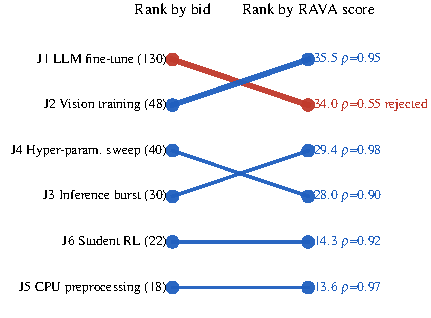
\includegraphics[width=\columnwidth]{figures/fig_rank.pdf}
\caption{Rank by bid versus rank by RAVA score in the worked example. J1 bids most but is unreliable and large; it drops below J2 and no longer fits.}
\label{fig:rank}
\end{figure}

\begin{figure*}[!t]
\centering
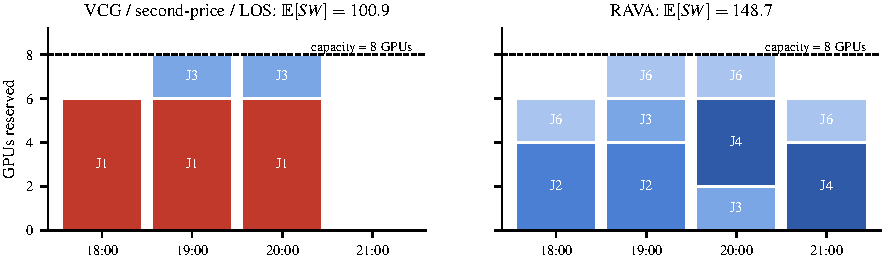
\includegraphics[width=\textwidth]{figures/fig_example.pdf}
\caption{GPU reservations in the worked example. Price-based auctions serve J1, which fails 45\% of the time; RAVA serves five reliable jobs. J5 uses no GPU and is not drawn.}
\label{fig:example}
\end{figure*}

\textbf{The same auction on a real Slurm cluster.} We ran this example through our Slurm broker (\cref{sec:slurm}) on a live Slurm 23.11 controller with one 8-GPU node and 20-second slots. The broker computed the same scores, winners and prices, to two decimals, in 161\,ms. Slurm started every winner 1--2\,s after its slot began (\cref{fig:slurm}). J4 was set to crash. Slurm recorded it as \texttt{FAILED}, so the broker charged nothing under $\kappa=0$ and lowered the tenant's reputation from 0.900 to 0.857 for the next epoch.

\begin{figure}[!t]
\centering
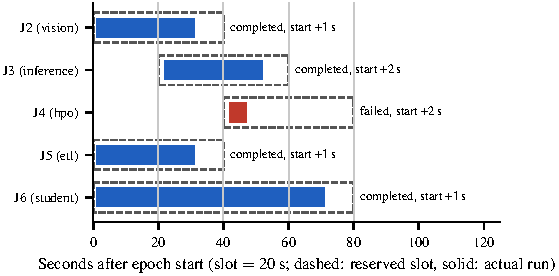
\includegraphics[width=\columnwidth]{figures/fig_slurm.pdf}
\caption{Live Slurm run of the worked example. Dashed boxes: slots reserved by RAVA. Bars: actual runs from Slurm's job-completion log. All jobs start within 2\,s of their slot; J4's real failure lowers its reputation.}
\label{fig:slurm}
\end{figure}

%=====================================================================
\section{Implementation}\label{sec:slurm}
%=====================================================================
\textbf{Simulator.} RAVA and all baselines share one placement engine, compiled with Numba~\cite{lam2015numba}. So the mechanisms differ only in how they rank and price. The LP bounds and exact VCG use HiGHS~\cite{huangfu2018} through SciPy~\cite{virtanen2020}. Before any new experiment, we checked that the new engine reproduces the welfare and payments of the earlier implementation exactly on the same workloads.

\textbf{Slurm broker.} The broker (about 90 lines of Python) works with an unmodified Slurm~\cite{yoo2003slurm}. It reads capacities from \texttt{scontrol show node}. It runs \cref{alg:alloc,alg:pay}. It submits each winner with \texttt{sbatch --begin=}$\langle$slot start$\rangle$, \texttt{--time}, \texttt{--gres=gpu:}$g$, \texttt{--cpus-per-task}, \texttt{--mem} and \texttt{--nodelist}. After the epoch it reads Slurm's job-completion log. It charges $p_i$ for \texttt{COMPLETED} jobs and $\kappa p_i$ otherwise, and updates \eqref{eq:rho}. Because RAVA's allocation already respects \eqref{eq:cap}, Slurm's own scheduler never has to delay a winner. Losers can be routed to a low-priority partition. A Kubernetes version would follow the same pattern through scheduling gates; we leave it to future work.

%=====================================================================
\section{Evaluation}\label{sec:eval}
%=====================================================================
\subsection{Methodology}
\textbf{Baselines.} First-price (bids shaded to 60--90\% of value), second-price greedy, LOS~\cite{lehmann2002}, G-VMPAC-II~\cite{nejad2015}, online primal-dual posted prices (OPD)~\cite{zhang2017ton,buchbinder2009}, McAfee~\cite{mcafee1992}, DRF~\cite{ghodsi2011}, overbooking by 10\% with eviction~\cite{qi2025ohtrust}, and exact VCG where it can be solved. OPD's price bounds were tuned on separate validation workloads, from ten percentile pairs; this did not change its ranking. All truthful mechanisms receive the dominant bids $\theta_i$.

\textbf{Statistics.} Every comparison is paired on the same instance. We report the mean per-instance gain, a 10{,}000-sample bootstrap 95\% CI~\cite{efron1979}, the Wilcoxon signed-rank test~\cite{wilcoxon1945} with Holm correction across all baselines in a table~\cite{holm1979}, and Cohen's $d_z$. ``Efficiency'' is welfare divided by an LP-relaxation upper bound of \eqref{eq:obj} that knows the true outcomes and pools server capacity; no mechanism can exceed it.

\textbf{Synthetic workloads.} 50 workloads for each $n\in\{40,80,120,160\}$, on 32 GPUs, 256 cores and 1{,}024\,GB over 24 hourly slots, with three job classes and 20\% unreliable tenants (run probability 0.3--0.6), as in our earlier study. Unless stated, $\kappa=0$, $\alpha=0.5$, $\gamma=0$ and $\lambda=0.2$.

\subsection{Synthetic Results}
\begin{figure}[!t]
\centering
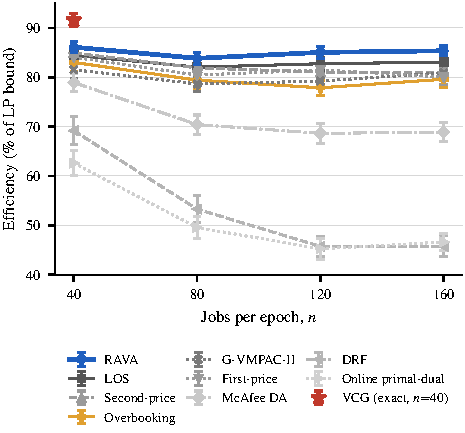
\includegraphics[width=\columnwidth]{figures/fig_efficiency.pdf}
\caption{Efficiency by market size (mean and 95\% CI, 50 workloads per size; VCG on 10 workloads at $n=40$). RAVA is the best polynomial-time mechanism at every size.}
\label{fig:eff}
\end{figure}

\begin{table*}[!t]
\caption{Synthetic Results at $n=120$ (50 Paired Workloads). Gain Is RAVA's Welfare Advantage Over Each Baseline.}\label{tab:main}
\centering\footnotesize
\begin{tabular}{@{}lccccccc@{}}
\toprule
Mechanism & Efficiency (\%) & RAVA's gain [95\% CI] & $p_{\rm Holm}$ & $d_z$ & Resources used (\%) & Resources wasted (\%) & Jobs served\\
\midrule
First-price & 81.5 & $+4.7\%$ [2.9, 6.5] & $<0.001$ & 0.72 & 48.7 & 31.2 & 35.7\\
Second-price & 81.0 & $+5.4\%$ [3.4, 7.5] & $<0.001$ & 0.76 & 48.2 & 31.6 & 35.8\\
LOS & 82.7 & $+2.9\%$ [1.6, 4.3] & $<0.001$ & 0.59 & 47.9 & 31.0 & 38.6\\
G-VMPAC-II & 79.2 & $+7.7\%$ [5.8, 9.7] & $<0.001$ & 1.13 & 45.6 & 29.7 & 48.4\\
Online primal-dual & 45.2 & $+93\%$ [84, 103] & $<0.001$ & 3.80 & 41.6 & 29.3 & 39.8\\
McAfee DA & 68.6 & $+25\%$ [22, 29] & $<0.001$ & 2.43 & 33.9 & 21.8 & 16.9\\
DRF & 45.7 & $+91\%$ [82, 100] & $<0.001$ & 3.59 & 45.0 & 30.7 & 44.2\\
Overbooking (10\%) & 77.9 & $+9.5\%$ [7.8, 11.3] & $<0.001$ & 1.57 & 52.4 & 34.5 & 41.0\\
\textbf{RAVA} & \textbf{85.0} & --- & --- & --- & 50.5 & 27.7 & 39.7\\
RAVA-E ($\gamma=1$) & 82.2 & $+3.7\%$ [2.1, 5.3] & $<0.001$ & 0.59 & \textbf{54.1} & \textbf{24.2} & 40.4\\
\bottomrule
\end{tabular}
\end{table*}

\Cref{fig:eff} and \cref{tab:main} show the main result. RAVA is the best polynomial-time mechanism at every size, at 83.8--86.1\% of the bound. It beats LOS by 2.2--3.0\%, with Holm $p\le0.028$ at every size, and wins 136 of 200 paired workloads (\cref{fig:scatter}). Overbooking trails here: in a pooled cluster its evictions cost more than the extra admissions gain. OPD processes jobs in arrival order, as an online mechanism must, so it cannot compete with batch mechanisms. Exact VCG remains 5.9\% (CI 3.6--8.6\%) better than RAVA at $n=40$, but it needs 129\,s per auction on average (max 335\,s), and at $n\ge80$ a single solve did not finish within 60\,s.

\begin{figure}[!t]
\centering
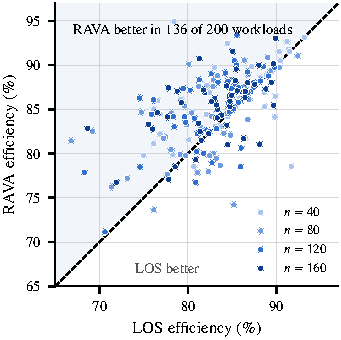
\includegraphics[width=0.8\columnwidth]{figures/fig_scatter.pdf}
\caption{All 200 synthetic workloads, RAVA against LOS. Dots above the diagonal favor RAVA.}
\label{fig:scatter}
\end{figure}

\begin{figure}[!t]
\centering
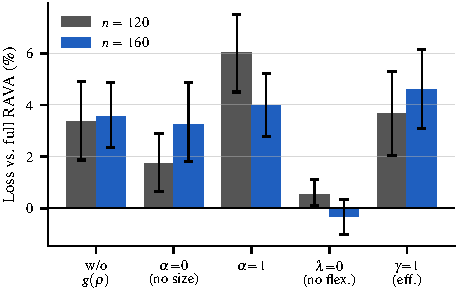
\includegraphics[width=\columnwidth]{figures/fig_ablation.pdf}
\caption{Ablation: welfare lost when one part of the score is changed (mean and bootstrap 95\% CI). Removing $g(\rho)$ costs 3.3--3.5\%; the flexibility bonus has no measurable effect under truthful windows.}
\label{fig:ablation}
\end{figure}

\textbf{Ablation} (\cref{fig:ablation}). Removing the reliability factor costs 3.3\% at $n=120$ and 3.5\% at $n=160$. Dropping the size weight ($\alpha=0$) costs 1.8--3.3\%, and $\alpha=1$ costs 4.0--6.0\%. Setting $\lambda=0$ makes no significant difference here, because every tenant already reports its true window. \Cref{sec:flex} tests the bonus where disclosure is a choice.

\subsection{Trace-Driven GPU Experiments (Microsoft Philly)}\label{sec:philly}
\textbf{Setup.} We replay the Philly job log~\cite{jeon2019philly} (117{,}325 jobs, 325 users, Aug.--Dec.\ 2017). Each epoch is one calendar day. The auction sells a 160-GPU sub-cluster of sixteen 8-GPU and sixteen 2-GPU servers over a 48-hour horizon. We draw 35\% of each day's jobs, which gives 465 jobs per epoch on average. From the trace we take each job's GPU count, gang size (jobs with more than 8 GPUs need several 8-GPU servers), run time (capped at 24\,h), submission hour, user, and \emph{real outcome}. Reputation uses only that user's earlier jobs. Efficiency $\eta$ is the user's mean measured GPU utilization on earlier jobs, computed from 44.7 million per-minute utilization records sampled every 10 minutes. Values (GPU-hours times log-normal user and job factors), deadline slack, and the reservation length of failed jobs (the user's median passed length) are synthetic. We tune RAVA's $(\alpha,\gamma)$ on the first 14 days (42 instances) and report the remaining 45 days (135 instances). A job counts as run only if its status is \texttt{Pass}.

\begin{figure*}[!t]
\centering
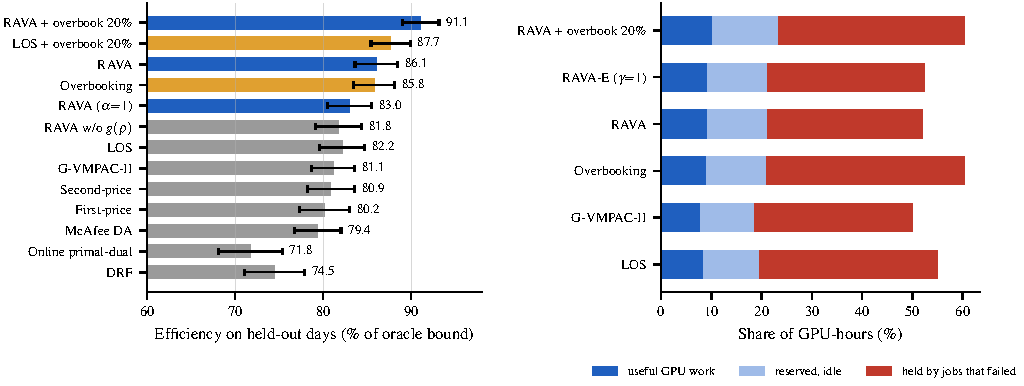
\includegraphics[width=\textwidth]{figures/fig_philly.pdf}
\caption{Philly GPU trace, 135 held-out instances. Left: efficiency (95\% CI). Right: where reserved GPU-hours go; red is capacity held by jobs that failed. RAVA ties overbooking on welfare but wastes less; RAVA plus overbooking is best.}
\label{fig:philly}
\end{figure*}

\begin{table}[!t]
\caption{Philly Trace: RAVA's Gain Over Each Baseline (135 Paired Instances, Holm-Corrected)}\label{tab:philly}
\centering\footnotesize\setlength{\tabcolsep}{2.6pt}
\begin{tabular}{@{}lcccc@{}}
\toprule
Baseline & Eff.\,(\%) & RAVA's gain [CI] & $p_{\rm Holm}$ & Lost\,(\%)\\
\midrule
First-price & 80.2 & $+10.4\%$ [6.5, 14.3] & $<0.001$ & 35.9\\
Second-price & 80.9 & $+8.8\%$ [5.4, 12.3] & $<0.001$ & 35.7\\
LOS & 82.2 & $+6.4\%$ [3.4, 9.4] & $<0.001$ & 35.5\\
G-VMPAC-II & 81.1 & $+7.5\%$ [4.6, 10.4] & $<0.001$ & 31.5\\
Online primal-dual & 71.8 & $+30.5\%$ [23.0, 38.5] & $<0.001$ & 31.4\\
McAfee DA & 79.4 & $+10.8\%$ [7.4, 14.6] & $<0.001$ & 30.3\\
DRF & 74.5 & $+22.8\%$ [17.2, 28.6] & $<0.001$ & 32.9\\
Overbooking & 85.8 & $+1.1\%$ [$-1.4$, 3.6] & 0.97 & 39.3\\
\midrule
\textbf{RAVA} & \textbf{86.1} & --- & --- & \textbf{30.9}\\
RAVA + overbook 20\% & \textbf{91.1} & $-5.8\%$ [$-7.1$, $-4.6$] & $<0.001$ & 36.9\\
\bottomrule
\end{tabular}
\\[2pt]{\scriptsize Lost: GPU-hours held by jobs that failed, as \% of capacity.}
\end{table}

\textbf{Results} (\cref{fig:philly}, \cref{tab:philly}). RAVA reaches 86.1\% of the oracle bound. It beats LOS by 6.4\% (Holm $p<0.001$) and every other price- or fairness-based mechanism by 7.5--30.5\%. It also holds much less GPU time for jobs that fail: 30.9\% of capacity, against 35.5\% for LOS. Overbooking is a strong alternative on this trace. Its welfare ties RAVA ($p=0.97$), but it reserves more capacity for jobs that then fail (39.3\%). The two ideas stack: RAVA's ranking with 20\% overbooking reaches 91.1\%, which is 5.0\% (CI 2.6--7.7\%, $p<0.001$) above LOS with the same overbooking. With the size rule of G-VMPAC-II ($\alpha=1$), adding $g(\rho)$ raises welfare by 3.4\% (bootstrap CI 0.7--6.2\%), but the Wilcoxon test is not significant ($p=0.32$), so we do not claim this effect. The tuned weights ($\alpha=0.25$, $\gamma=0.5$) match the defaults ($+0.5\%$, n.s.). On measured GPU utilization, $\gamma=0.5$ raises useful GPU work from 9.15\% to 9.32\% of capacity, a small effect.

\textbf{When RAVA does not help.} The Philly log also has \texttt{Killed} jobs, which users or the system stopped. If we count them as successes, consistently in both history and outcome, RAVA's gain over LOS falls to $-0.02\%$ (CI $-2.8$ to $2.6\%$). User history predicts outcomes equally well under both definitions (AUC 0.84 and 0.85). What changes is how much capacity failures hold: 57\% of GPU-hours with Killed counted as failure, but only 31\% with Killed counted as success. RAVA pays off only when failed reservations hold a large share of capacity.

\subsection{Deposits and Beliefs}
\begin{figure*}[!t]
\centering
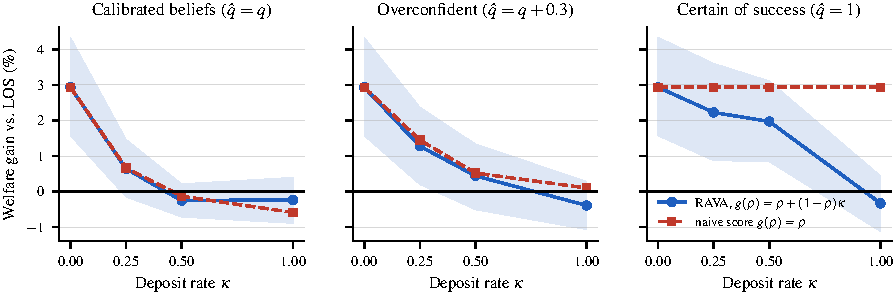
\includegraphics[width=\textwidth]{figures/fig_kappa.pdf}
\caption{Effect of the deposit rate $\kappa$ under three belief models ($n=120$, 50 workloads; band: 95\% CI for RAVA). With calibrated tenants the deposit already prices risk. With overconfident tenants only the operator's reputation does, and the correct factor depends on beliefs, as \cref{prop:rank} predicts.}
\label{fig:kappa}
\end{figure*}

\Cref{fig:kappa} tests \cref{prop:rank}. At $\kappa=0$ all variants coincide and RAVA gains 2.9\% over LOS. With calibrated tenants, larger deposits let tenants price their own risk. RAVA's gain then falls to zero, and the naive factor double-counts risk: at $\kappa=1$ it is 0.6\% below LOS, while RAVA is level ($-0.2\%$, n.s.). With tenants who are certain they will succeed, the deposit has no effect on bids, so only the operator's reputation carries risk. Here the naive factor keeps the full 2.9\% gain, while $g_\kappa$ discounts the reputation and loses it as $\kappa\to1$. This is \cref{cor:kappa0} in action: when tenants' calibration is unknown, $\kappa=0$ is the safe choice.

\subsection{Unreliable and Adversarial Users}
\begin{figure}[!t]
\centering
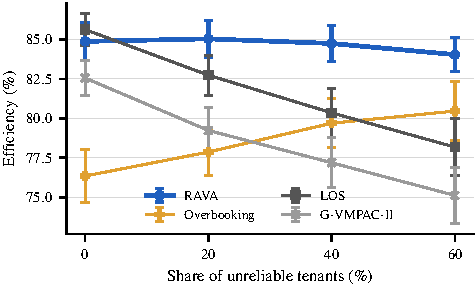
\includegraphics[width=\columnwidth]{figures/fig_bad.pdf}
\caption{Efficiency as the share of unreliable tenants grows ($n=120$, 50 workloads, 95\% CI).}
\label{fig:bad}
\end{figure}

\textbf{More unreliable users} (\cref{fig:bad}). With no unreliable tenants, RAVA is level with LOS ($-0.8\%$, n.s.). Its gain rises to 2.9\%, 5.8\% and 8.2\% at 20\%, 40\% and 60\% unreliable tenants. RAVA's efficiency stays at 84.0--85.0\% while LOS falls to 78.2\%. Overbooking improves as no-shows increase but stays 5.1--11.7\% behind RAVA.

\begin{figure}[!t]
\centering
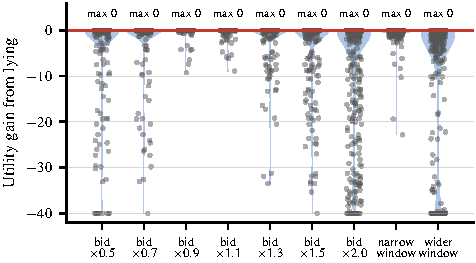
\includegraphics[width=\columnwidth]{figures/fig_regret.pdf}
\caption{Empirical single-epoch regret: utility gained by lying, over 600 tenants per deviation ($\kappa=0.5$). No deviation ever gains.}
\label{fig:regret}
\end{figure}

\textbf{Lying does not pay} (\cref{fig:regret}). We took 600 tenants and tried bids from 0.5 to 2 times $\theta_i$, narrower windows (491 cases) and later deadlines. Across 5{,}291 deviations the largest gain was exactly 0, as \cref{thm:dsic} states. For the multi-epoch incentive, one reliable tenant overbid by 30\% in its first epoch to buy reputation. Over the next 20 epochs ($\delta=0.9$) its discounted gain averaged $-0.42\pm0.45$, against a mean job value of 30.2. Only 4\% of 100 trials gained anything, consistent with \cref{thm:multi}.

\begin{figure*}[!t]
\centering
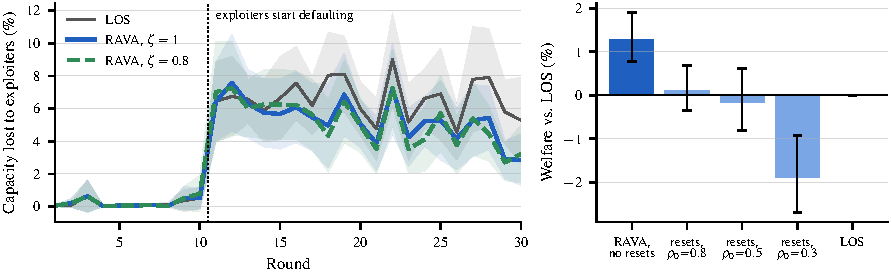
\includegraphics[width=\textwidth]{figures/fig_adversary.pdf}
\caption{Left: build-then-exploit. 10\% of tenants behave well for 10 epochs and then default 90\% of the time; RAVA cuts the capacity they waste by 18\%. Right: whitewashing. Tenants that reset their identity erase RAVA's 1.3\% gain, and a harsh newcomer prior only hurts honest newcomers. Bars: total welfare over 30 epochs relative to LOS (20 runs, 95\% CI).}
\label{fig:adv}
\end{figure*}

\textbf{Build-then-exploit} (\cref{fig:adv}, left). After the switch, LOS keeps admitting the exploiters. RAVA lowers their reputation after a few defaults and cuts the capacity they waste by 18.0\% (CI 11.2--24.1\%, $p<0.001$). Forgetting ($\zeta=0.8$) helps a little more in this short horizon, as \cref{prop:exploit} predicts; its benefit grows with history length.

\textbf{Whitewashing} (\cref{fig:adv}, right). Without identity resets, RAVA earns 1.3\% more than LOS over 30 epochs. If unreliable tenants reset their identity whenever their reputation falls below the newcomer prior, this gain vanishes ($+0.1\%$, n.s.). Lowering the prior to 0.3 removes the incentive (\cref{prop:white}), but it penalizes honest newcomers and costs 1.9\%. In practice RAVA therefore needs identities that are costly to replace, such as institutional accounts or an entry deposit.

\subsection{Scalability}
\begin{figure*}[!t]
\centering
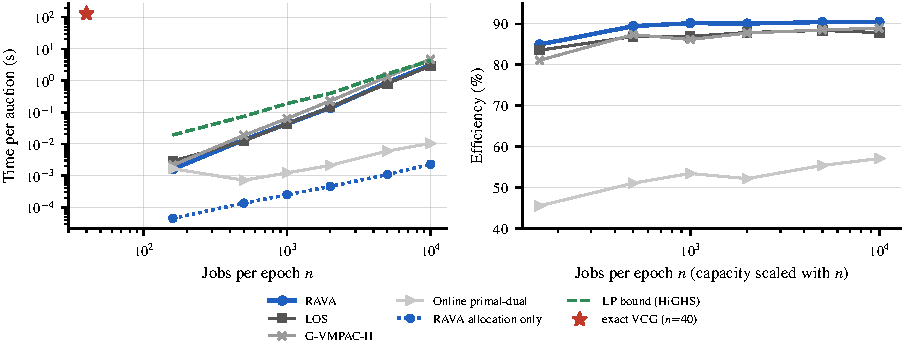
\includegraphics[width=\textwidth]{figures/fig_scale.pdf}
\caption{Scaling to 10{,}000 jobs with capacity scaled in proportion. Left: time per auction including all critical payments. Right: efficiency.}
\label{fig:scale}
\end{figure*}

We grew markets from 160 to 10{,}000 jobs, with capacity scaled in proportion (\cref{fig:scale}). A full RAVA auction, with all critical payments, takes 1.6\,ms at 160 jobs, 43\,ms at 1{,}000 and 3.1\,s at 10{,}000; allocation alone takes 2.3\,ms at 10{,}000. Efficiency rises from 85.0\% to 90.5\% as markets grow, and RAVA stays 2.5\% (CI 2.3--2.9\%) above LOS for $n\ge2{,}000$, winning all 8 large instances. The LP bound itself takes 4.3\,s at 10{,}000 jobs.

\subsection{Flexibility and Efficiency}\label{sec:flex}
\begin{figure}[!t]
\centering
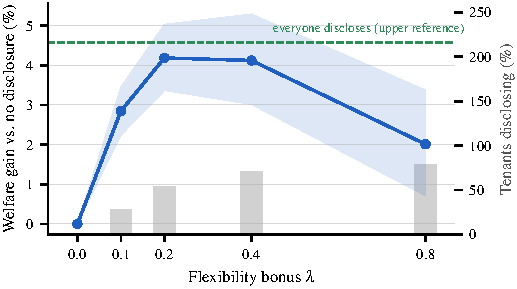
\includegraphics[width=\columnwidth]{figures/fig_flex.pdf}
\caption{Disclosure of slack. Tenant $i$ loses up to $c_i\sim U(0,0.3)$ of its value if started late and discloses its window only if $\lambda\varphi_i\ge c_i/2$. Bars: share disclosing; line: welfare gain over no disclosure, counting delay losses.}
\label{fig:flex}
\end{figure}

\textbf{Flexibility.} The earlier ablation assumed honest windows. In practice, revealing slack has a cost: a job may start later. We model tenant $i$ as losing up to a share $c_i\sim U(0,0.3)$ of its value if it starts at the end of its window. It discloses its window only if the bonus outweighs half that loss (\cref{fig:flex}). With $\lambda=0$ nobody discloses. With $\lambda=0.2$, 54\% disclose and welfare rises by 4.2\%, close to the 4.6\% gained if everyone disclosed. A large bonus ($\lambda=0.8$) distorts the ranking and returns only 2.0\%. This behavioral model is an assumption; \cref{thm:dsic} covers only truthful windows.

\textbf{Efficiency.} \Cref{fig:gpuday} shows where GPU time goes in the synthetic cluster. RAVA cuts the GPU time lost to no-shows from 12\% to 8\%. The efficiency weight $\gamma$ trades welfare for utilization (\cref{fig:heatmap}). On Philly's measured utilization the same dial has only a small effect.

\begin{figure*}[!t]
\centering
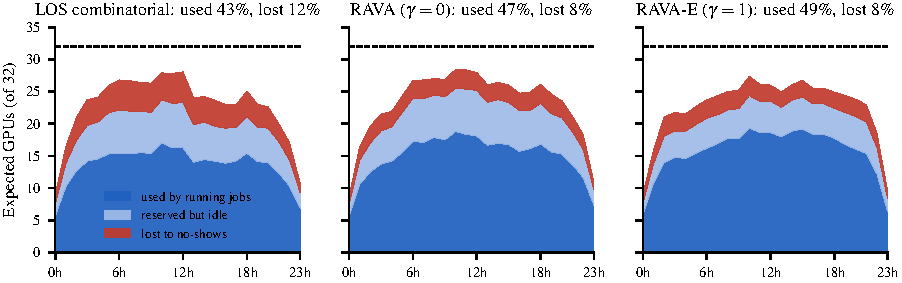
\includegraphics[width=\textwidth]{figures/fig_gpu_day.pdf}
\caption{Expected GPU use over one day, synthetic, 120 jobs (mean of 20 workloads): useful work, reserved but idle, and lost to no-shows.}
\label{fig:gpuday}
\end{figure*}

\begin{figure*}[!t]
\centering
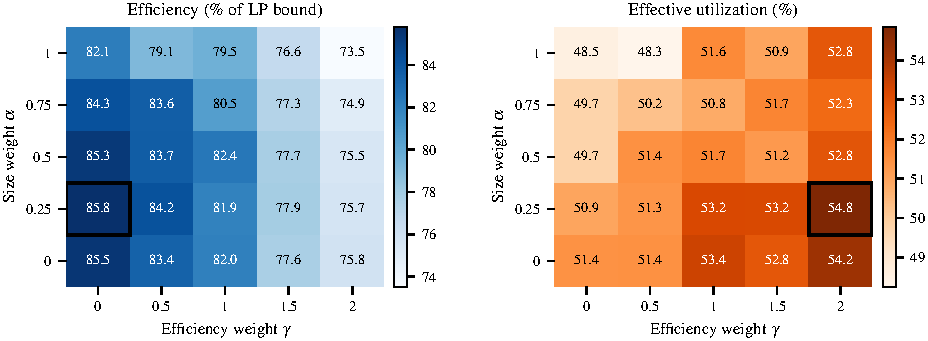
\includegraphics[width=\textwidth]{figures/fig_heatmap.pdf}
\caption{Size weight $\alpha$ and efficiency weight $\gamma$ (synthetic, 120 jobs). Value peaks at small $\gamma$ and $\alpha\le0.5$; utilization peaks at large $\gamma$.}
\label{fig:heatmap}
\end{figure*}

\subsection{Overall Comparison}
\begin{figure}[!t]
\centering
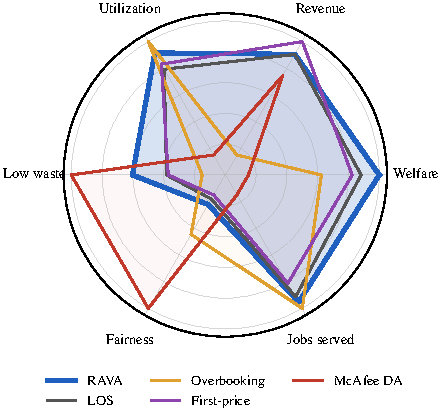
\includegraphics[width=0.88\columnwidth]{figures/fig_radar.pdf}
\caption{Six measures at once (synthetic, 120 jobs; the outer edge is the best mechanism on each measure).}
\label{fig:radar}
\end{figure}
\Cref{fig:radar} sums up the synthetic results. RAVA leads on welfare and is near the top on utilization and jobs served. First-price earns the most revenue. McAfee appears fair and low-waste only because it serves the fewest jobs.

\subsection{Threats to Validity}
Values, deadline slack and the reservation length of failed jobs are synthetic even in the trace study. The sub-cluster and sampling rate are our choices. Epochs are independent days, with no carry-over of long jobs. The results depend on whether \texttt{Killed} jobs count as failures. First-price shading is assumed, not solved. The flexibility study uses a behavioral model. The Slurm run uses one node with placeholder GPU devices. It shows that the broker works end to end, not that RAVA performs well in production.

%=====================================================================
\section{Conclusion and Future Work}\label{sec:concl}
%=====================================================================
RAVA prices the risk that a winning job will not run, and keeps honest bidding dominant. A clear settlement rule leads to the right reliability factor, $g_\kappa(\rho)=\rho+(1-\rho)\kappa$, and shows when deposits and reputation substitute for each other. Over many epochs honest bidding stays nearly optimal, and forgetting bounds the damage from users who exploit a good reputation. On real Philly GPU jobs RAVA beats every price-based baseline, ties overbooking, and combines with overbooking to reach 91.1\% of an oracle bound. It scales to 10{,}000 jobs and runs on Slurm. Its gain depends on how much capacity failures hold: with few resources lost, it brings little.

\textbf{Future work.} 1)~Deploy the broker on a production Slurm partition and build a Kubernetes version. 2)~Model long jobs that span epochs, and add preemption. 3)~Combine RAVA with overbooking in one truthful mechanism. 4)~Make identities costly to defeat whitewashing. 5)~Learn tenants' calibration so that $\kappa>0$ can be used safely. 6)~Pack better at the same speed, for example with LP rounding~\cite{lavi2011}. 7)~Test exact solvers, including quantum annealing on the QUBO form~\cite{lucas2014,farhi2014}, as offline benchmarks only.

\bibliographystyle{IEEEtran}
\bibliography{refs}

\appendices
\section{Reproducibility}
The artifact is an installable Python package (\texttt{pip install -e .}) with a command-line tool. The package \texttt{rava} mirrors the paper. \texttt{model}, \texttt{reputation} and \texttt{settlement} implement Section~III. \texttt{placement} and \texttt{mechanism} implement \cref{alg:alloc,alg:pay}. \texttt{theory} implements Section~V. \texttt{baselines} and \texttt{bounds} hold the comparators. \texttt{experiments} produces every run. \texttt{analysis} computes every number and figure from the raw results, and \texttt{integrations.slurm\_broker} is the Slurm broker. A test suite of 44 tests checks monotonicity, exact critical prices, the absence of profitable deviations, the worked example, the closed-form results and regression against the stored results. \texttt{rava check} compares the stored results with every number quoted in this paper. Random seeds are fixed: synthetic workload $s$ at size $n$ uses seed $1000n+s$, and Philly epochs use seeds 1--3. \texttt{scripts/run\_all.sh} reruns everything in about an hour on two cores.

\section{Philly Preprocessing}
We keep jobs with at least one attempt that records its GPUs (111{,}549 of 117{,}325). Run time runs from the first attempt's start to the last attempt's end. Jobs with more than 8 GPUs are placed on $\lceil g/8\rceil$ 8-GPU servers. A failed job reserves the median run time of the same user's passed jobs with the same GPU count, falling back to the median over all users. Reputation uses a Beta(3,1) prior, which matches the trace's 76\% pass rate.

\begin{IEEEbiographynophoto}{Firstname Lastname}
received the Ph.D.\ degree in computer science. Research interests include algorithmic game theory, distributed computing and cluster scheduling.
\end{IEEEbiographynophoto}
\end{document}
